\documentclass[1p]{elsarticle_modified}
%\bibliographystyle{elsarticle-num}

%\usepackage[colorlinks]{hyperref}
%\usepackage{abbrmath_seonhwa} %\Abb, \Ascr, \Acal ,\Abf, \Afrak
\usepackage{amsfonts}
\usepackage{amssymb}
\usepackage{amsmath}
\usepackage{amsthm}
\usepackage{scalefnt}
\usepackage{amsbsy}
\usepackage{kotex}
\usepackage{caption}
\usepackage{subfig}
\usepackage{color}
\usepackage{graphicx}
\usepackage{xcolor} %% white, black, red, green, blue, cyan, magenta, yellow
\usepackage{float}
\usepackage{setspace}
\usepackage{hyperref}

\usepackage{tikz}
\usetikzlibrary{arrows}

\usepackage{multirow}
\usepackage{array} % fixed length table
\usepackage{hhline}

%%%%%%%%%%%%%%%%%%%%%
\makeatletter
\renewcommand*\env@matrix[1][\arraystretch]{%
	\edef\arraystretch{#1}%
	\hskip -\arraycolsep
	\let\@ifnextchar\new@ifnextchar
	\array{*\c@MaxMatrixCols c}}
\makeatother %https://tex.stackexchange.com/questions/14071/how-can-i-increase-the-line-spacing-in-a-matrix
%%%%%%%%%%%%%%%

\usepackage[normalem]{ulem}

\newcommand{\msout}[1]{\ifmmode\text{\sout{\ensuremath{#1}}}\else\sout{#1}\fi}
%SOURCE: \msout is \stkout macro in https://tex.stackexchange.com/questions/20609/strikeout-in-math-mode

\newcommand{\cancel}[1]{
	\ifmmode
	{\color{red}\msout{#1}}
	\else
	{\color{red}\sout{#1}}
	\fi
}

\newcommand{\add}[1]{
	{\color{blue}\uwave{#1}}
}

\newcommand{\replace}[2]{
	\ifmmode
	{\color{red}\msout{#1}}{\color{blue}\uwave{#2}}
	\else
	{\color{red}\sout{#1}}{\color{blue}\uwave{#2}}
	\fi
}

\newcommand{\Sol}{\mathcal{S}} %segment
\newcommand{\D}{D} %diagram
\newcommand{\A}{\mathcal{A}} %arc


%%%%%%%%%%%%%%%%%%%%%%%%%%%%%5 test

\def\sl{\operatorname{\textup{SL}}(2,\Cbb)}
\def\psl{\operatorname{\textup{PSL}}(2,\Cbb)}
\def\quan{\mkern 1mu \triangleright \mkern 1mu}

\theoremstyle{definition}
\newtheorem{thm}{Theorem}[section]
\newtheorem{prop}[thm]{Proposition}
\newtheorem{lem}[thm]{Lemma}
\newtheorem{ques}[thm]{Question}
\newtheorem{cor}[thm]{Corollary}
\newtheorem{defn}[thm]{Definition}
\newtheorem{exam}[thm]{Example}
\newtheorem{rmk}[thm]{Remark}
\newtheorem{alg}[thm]{Algorithm}

\newcommand{\I}{\sqrt{-1}}
\begin{document}

%\begin{frontmatter}
%
%\title{Boundary parabolic representations of knots up to 8 crossings}
%
%%% Group authors per affiliation:
%\author{Yunhi Cho} 
%\address{Department of Mathematics, University of Seoul, Seoul, Korea}
%\ead{yhcho@uos.ac.kr}
%
%
%\author{Seonhwa Kim} %\fnref{s_kim}}
%\address{Center for Geometry and Physics, Institute for Basic Science, Pohang, 37673, Korea}
%\ead{ryeona17@ibs.re.kr}
%
%\author{Hyuk Kim}
%\address{Department of Mathematical Sciences, Seoul National University, Seoul 08826, Korea}
%\ead{hyukkim@snu.ac.kr}
%
%\author{Seokbeom Yoon}
%\address{Department of Mathematical Sciences, Seoul National University, Seoul, 08826,  Korea}
%\ead{sbyoon15@snu.ac.kr}
%
%\begin{abstract}
%We find all boundary parabolic representation of knots up to 8 crossings.
%
%\end{abstract}
%\begin{keyword}
%    \MSC[2010] 57M25 
%\end{keyword}
%
%\end{frontmatter}

%\linenumbers
%\tableofcontents
%
\newcommand\colored[1]{\textcolor{white}{\rule[-0.35ex]{0.8em}{1.4ex}}\kern-0.8em\color{red} #1}%
%\newcommand\colored[1]{\textcolor{white}{ #1}\kern-2.17ex	\textcolor{white}{ #1}\kern-1.81ex	\textcolor{white}{ #1}\kern-2.15ex\color{red}#1	}

{\Large $\underline{12a_{0617}~(K12a_{0617})}$}

\setlength{\tabcolsep}{10pt}
\renewcommand{\arraystretch}{1.6}
\vspace{1cm}\begin{tabular}{m{100pt}>{\centering\arraybackslash}m{274pt}}
\multirow{5}{120pt}{
	\centering
	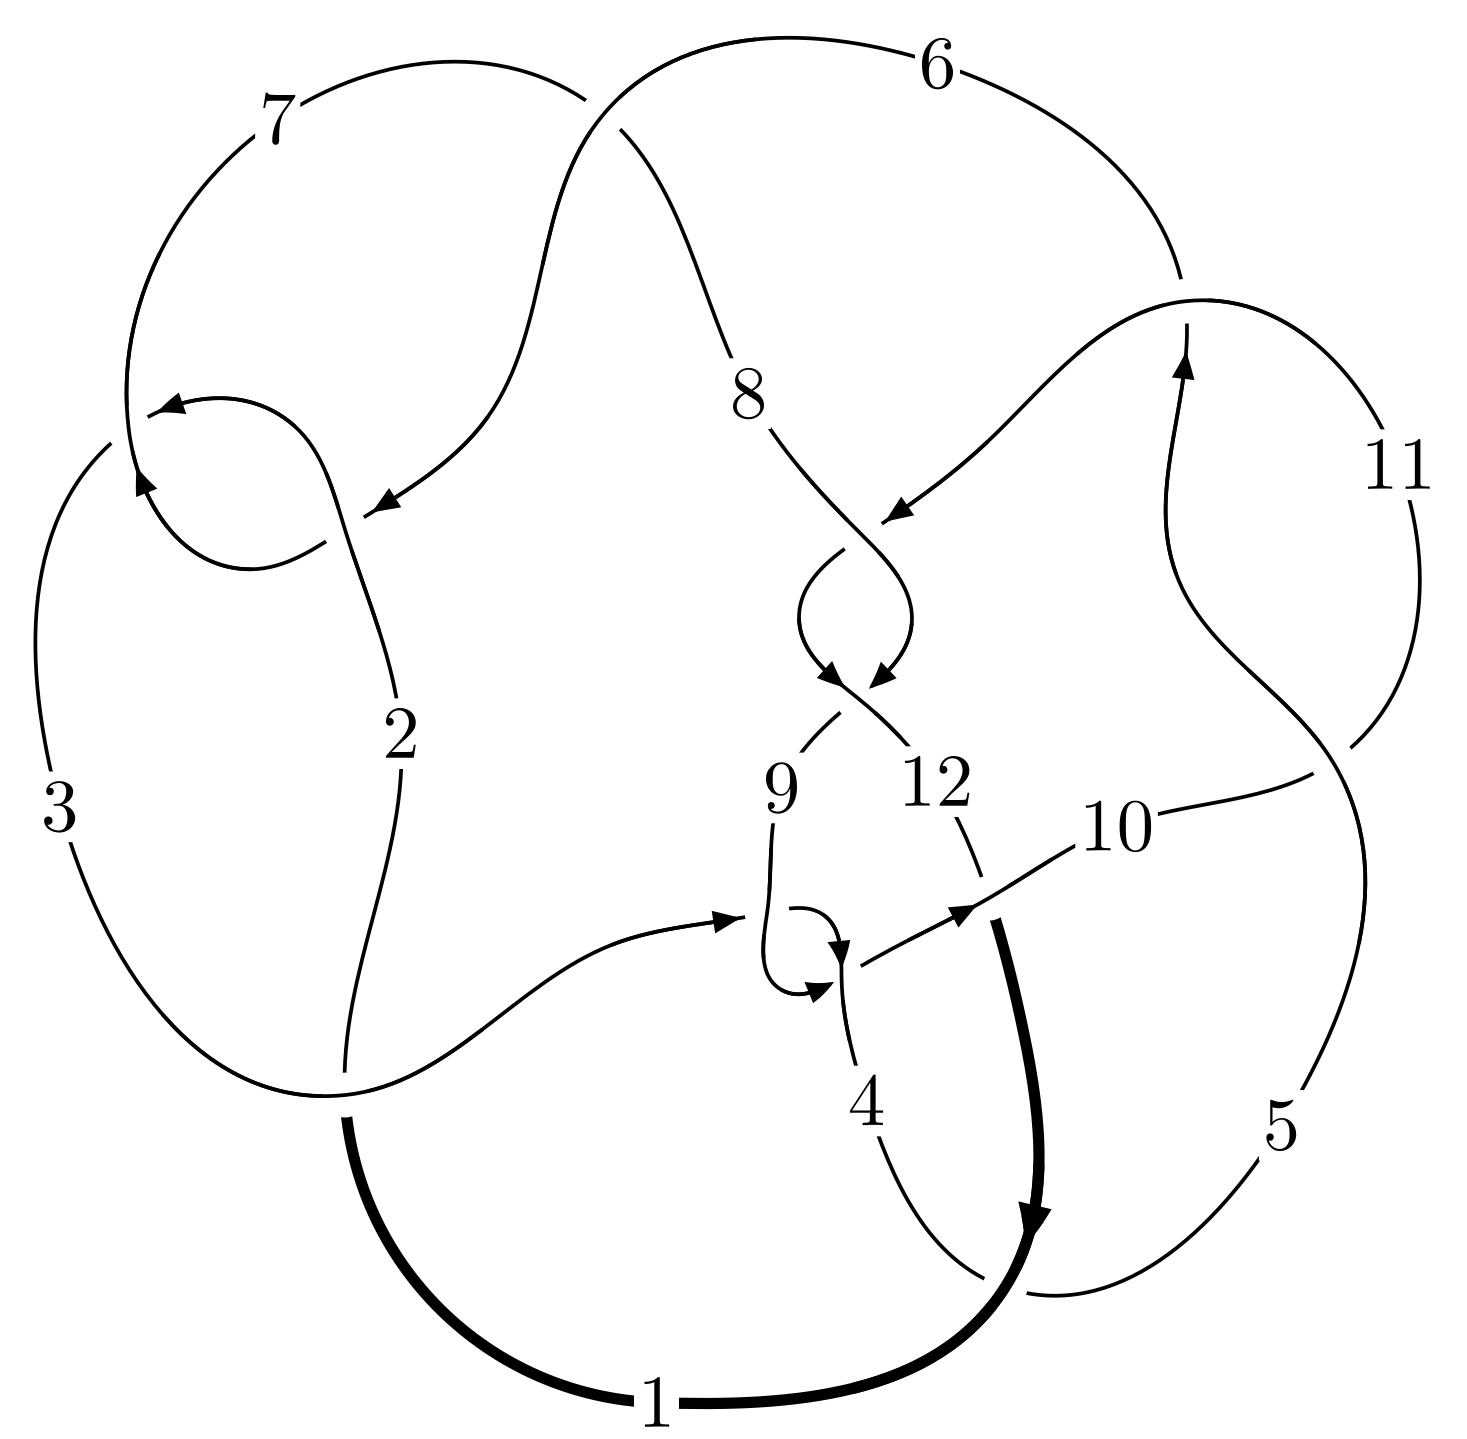
\includegraphics[width=112pt]{../../../GIT/diagram.site/Diagrams/png/1418_12a_0617.png}\\
\ \ \ A knot diagram\footnotemark}&
\allowdisplaybreaks
\textbf{Linearized knot diagam} \\
\cline{2-2}
 &
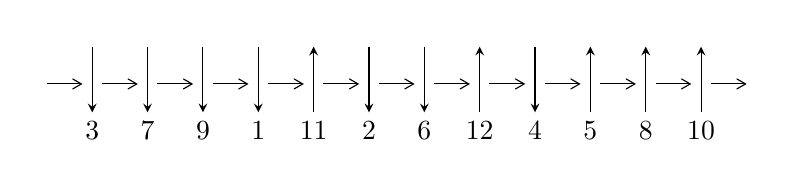
\begin{tikzpicture}[x=20pt, y=17pt]
	% nodes
	\node (C0) at (0, 0) {};
	\node (C1) at (1, 0) {};
	\node (C1U) at (1, +1) {};
	\node (C1D) at (1, -1) {3};

	\node (C2) at (2, 0) {};
	\node (C2U) at (2, +1) {};
	\node (C2D) at (2, -1) {7};

	\node (C3) at (3, 0) {};
	\node (C3U) at (3, +1) {};
	\node (C3D) at (3, -1) {9};

	\node (C4) at (4, 0) {};
	\node (C4U) at (4, +1) {};
	\node (C4D) at (4, -1) {1};

	\node (C5) at (5, 0) {};
	\node (C5U) at (5, +1) {};
	\node (C5D) at (5, -1) {11};

	\node (C6) at (6, 0) {};
	\node (C6U) at (6, +1) {};
	\node (C6D) at (6, -1) {2};

	\node (C7) at (7, 0) {};
	\node (C7U) at (7, +1) {};
	\node (C7D) at (7, -1) {6};

	\node (C8) at (8, 0) {};
	\node (C8U) at (8, +1) {};
	\node (C8D) at (8, -1) {12};

	\node (C9) at (9, 0) {};
	\node (C9U) at (9, +1) {};
	\node (C9D) at (9, -1) {4};

	\node (C10) at (10, 0) {};
	\node (C10U) at (10, +1) {};
	\node (C10D) at (10, -1) {5};

	\node (C11) at (11, 0) {};
	\node (C11U) at (11, +1) {};
	\node (C11D) at (11, -1) {8};

	\node (C12) at (12, 0) {};
	\node (C12U) at (12, +1) {};
	\node (C12D) at (12, -1) {10};
	\node (C13) at (13, 0) {};

	% arrows
	\draw[->,>={angle 60}]
	(C0) edge (C1) (C1) edge (C2) (C2) edge (C3) (C3) edge (C4) (C4) edge (C5) (C5) edge (C6) (C6) edge (C7) (C7) edge (C8) (C8) edge (C9) (C9) edge (C10) (C10) edge (C11) (C11) edge (C12) (C12) edge (C13) ;	\draw[->,>=stealth]
	(C1U) edge (C1D) (C2U) edge (C2D) (C3U) edge (C3D) (C4U) edge (C4D) (C5D) edge (C5U) (C6U) edge (C6D) (C7U) edge (C7D) (C8D) edge (C8U) (C9U) edge (C9D) (C10D) edge (C10U) (C11D) edge (C11U) (C12D) edge (C12U) ;
	\end{tikzpicture} \\
\hhline{~~} \\& 
\textbf{Solving Sequence} \\ \cline{2-2} 
 &
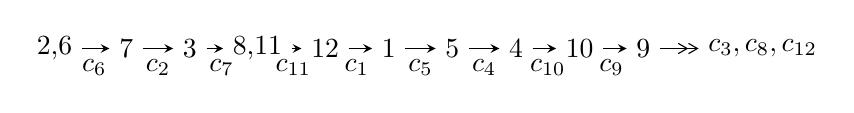
\begin{tikzpicture}[x=23pt, y=7pt]
	% node
	\node (A0) at (-1/8, 0) {2,6};
	\node (A1) at (1, 0) {7};
	\node (A2) at (2, 0) {3};
	\node (A3) at (49/16, 0) {8,11};
	\node (A4) at (33/8, 0) {12};
	\node (A5) at (41/8, 0) {1};
	\node (A6) at (49/8, 0) {5};
	\node (A7) at (57/8, 0) {4};
	\node (A8) at (65/8, 0) {10};
	\node (A9) at (73/8, 0) {9};
	\node (C1) at (1/2, -1) {$c_{6}$};
	\node (C2) at (3/2, -1) {$c_{2}$};
	\node (C3) at (5/2, -1) {$c_{7}$};
	\node (C4) at (29/8, -1) {$c_{11}$};
	\node (C5) at (37/8, -1) {$c_{1}$};
	\node (C6) at (45/8, -1) {$c_{5}$};
	\node (C7) at (53/8, -1) {$c_{4}$};
	\node (C8) at (61/8, -1) {$c_{10}$};
	\node (C9) at (69/8, -1) {$c_{9}$};
	\node (A10) at (11, 0) {$c_{3},c_{8},c_{12}$};

	% edge
	\draw[->,>=stealth]	
	(A0) edge (A1) (A1) edge (A2) (A2) edge (A3) (A3) edge (A4) (A4) edge (A5) (A5) edge (A6) (A6) edge (A7) (A7) edge (A8) (A8) edge (A9) ;
	\draw[->>,>={angle 60}]	
	(A9) edge (A10);
\end{tikzpicture} \\ 

\end{tabular} \\

\footnotetext{
The image of knot diagram is generated by the software ``\textbf{Draw programme}" developed by Andrew Bartholomew(\url{http://www.layer8.co.uk/maths/draw/index.htm\#Running-draw}), where we modified some parts for our purpose(\url{https://github.com/CATsTAILs/LinksPainter}).
}\phantom \\ \newline 
\centering \textbf{Ideals for irreducible components\footnotemark of $X_{\text{par}}$} 
 
\begin{align*}
I^u_{1}&=\langle 
4.14855\times10^{164} u^{108}+9.91104\times10^{164} u^{107}+\cdots+3.18106\times10^{164} b-5.08463\times10^{164},\\
\phantom{I^u_{1}}&\phantom{= \langle  }6.17984\times10^{164} u^{108}+1.13910\times10^{165} u^{107}+\cdots+1.59053\times10^{164} a-5.91043\times10^{165},\;u^{109}+2 u^{108}+\cdots- u+1\rangle \\
I^u_{2}&=\langle 
u^{19}+u^{18}+\cdots+b-4,\;-3 u^{19}+u^{18}+\cdots+a+7,\;u^{20}-4 u^{18}+\cdots-2 u+1\rangle \\
I^u_{3}&=\langle 
b-1,\;a,\;u-1\rangle \\
I^u_{4}&=\langle 
b^2- b-1,\;a-1,\;u+1\rangle \\
\\
\end{align*}
\raggedright * 4 irreducible components of $\dim_{\mathbb{C}}=0$, with total 132 representations.\\
\footnotetext{All coefficients of polynomials are rational numbers. But the coefficients are sometimes approximated in decimal forms when there is not enough margin.}
\newpage
\renewcommand{\arraystretch}{1}
\centering \section*{I. $I^u_{1}= \langle 4.15\times10^{164} u^{108}+9.91\times10^{164} u^{107}+\cdots+3.18\times10^{164} b-5.08\times10^{164},\;6.18\times10^{164} u^{108}+1.14\times10^{165} u^{107}+\cdots+1.59\times10^{164} a-5.91\times10^{165},\;u^{109}+2 u^{108}+\cdots- u+1 \rangle$}
\flushleft \textbf{(i) Arc colorings}\\
\begin{tabular}{m{7pt} m{180pt} m{7pt} m{180pt} }
\flushright $a_{2}=$&$\begin{pmatrix}0\\u\end{pmatrix}$ \\
\flushright $a_{6}=$&$\begin{pmatrix}1\\0\end{pmatrix}$ \\
\flushright $a_{7}=$&$\begin{pmatrix}1\\u^2\end{pmatrix}$ \\
\flushright $a_{3}=$&$\begin{pmatrix}- u\\- u^3+u\end{pmatrix}$ \\
\flushright $a_{8}=$&$\begin{pmatrix}- u^2+1\\u^2\end{pmatrix}$ \\
\flushright $a_{11}=$&$\begin{pmatrix}-3.88539 u^{108}-7.16176 u^{107}+\cdots+83.5734 u+37.1601\\-1.30414 u^{108}-3.11564 u^{107}+\cdots+2.90688 u+1.59841\end{pmatrix}$ \\
\flushright $a_{12}=$&$\begin{pmatrix}-5.74724 u^{108}-12.0466 u^{107}+\cdots+79.9400 u+36.7275\\-2.82416 u^{108}-7.12730 u^{107}+\cdots+4.15601 u+3.73114\end{pmatrix}$ \\
\flushright $a_{1}=$&$\begin{pmatrix}u^3\\u^5- u^3+u\end{pmatrix}$ \\
\flushright $a_{5}=$&$\begin{pmatrix}-7.34366 u^{108}-15.8462 u^{107}+\cdots+88.9383 u+26.8680\\-6.27613 u^{108}-16.6099 u^{107}+\cdots-1.72407 u+7.60193\end{pmatrix}$ \\
\flushright $a_{4}=$&$\begin{pmatrix}-8.04051 u^{108}-17.6315 u^{107}+\cdots+89.0488 u+27.8585\\-7.00281 u^{108}-18.8717 u^{107}+\cdots-6.88071 u+8.02606\end{pmatrix}$ \\
\flushright $a_{10}=$&$\begin{pmatrix}-12.2999 u^{108}-29.7434 u^{107}+\cdots+40.7832 u+37.0813\\-4.77830 u^{108}-12.1689 u^{107}+\cdots+10.2999 u+7.68948\end{pmatrix}$ \\
\flushright $a_{9}=$&$\begin{pmatrix}0.938066 u^{108}-0.178675 u^{107}+\cdots-64.8311 u-6.66318\\4.49012 u^{108}+12.5916 u^{107}+\cdots+9.61880 u-5.02522\end{pmatrix}$\\&\end{tabular}
\flushleft \textbf{(ii) Obstruction class $= -1$}\\~\\
\flushleft \textbf{(iii) Cusp Shapes $= 43.5911 u^{108}+118.988 u^{107}+\cdots+1.05585 u-49.2425$}\\~\\
\newpage\renewcommand{\arraystretch}{1}
\flushleft \textbf{(iv) u-Polynomials at the component}\newline \\
\begin{tabular}{m{50pt}|m{274pt}}
Crossings & \hspace{64pt}u-Polynomials at each crossing \\
\hline $$\begin{aligned}c_{1},c_{7}\end{aligned}$$&$\begin{aligned}
&u^{109}+32 u^{108}+\cdots+55 u+1
\end{aligned}$\\
\hline $$\begin{aligned}c_{2},c_{6}\end{aligned}$$&$\begin{aligned}
&u^{109}-2 u^{108}+\cdots- u-1
\end{aligned}$\\
\hline $$\begin{aligned}c_{3},c_{9}\end{aligned}$$&$\begin{aligned}
&u^{109}- u^{108}+\cdots+856 u+293
\end{aligned}$\\
\hline $$\begin{aligned}c_{4}\end{aligned}$$&$\begin{aligned}
&u^{109}-2 u^{108}+\cdots-108 u+52
\end{aligned}$\\
\hline $$\begin{aligned}c_{5},c_{10}\end{aligned}$$&$\begin{aligned}
&u^{109}+u^{108}+\cdots+48996 u+21519
\end{aligned}$\\
\hline $$\begin{aligned}c_{8},c_{11}\end{aligned}$$&$\begin{aligned}
&u^{109}- u^{108}+\cdots+18267 u-793
\end{aligned}$\\
\hline $$\begin{aligned}c_{12}\end{aligned}$$&$\begin{aligned}
&u^{109}+13 u^{108}+\cdots-28 u-1
\end{aligned}$\\
\hline
\end{tabular}\\~\\
\newpage\renewcommand{\arraystretch}{1}
\flushleft \textbf{(v) Riley Polynomials at the component}\newline \\
\begin{tabular}{m{50pt}|m{274pt}}
Crossings & \hspace{64pt}Riley Polynomials at each crossing \\
\hline $$\begin{aligned}c_{1},c_{7}\end{aligned}$$&$\begin{aligned}
&y^{109}+100 y^{108}+\cdots+307 y-1
\end{aligned}$\\
\hline $$\begin{aligned}c_{2},c_{6}\end{aligned}$$&$\begin{aligned}
&y^{109}-32 y^{108}+\cdots+55 y-1
\end{aligned}$\\
\hline $$\begin{aligned}c_{3},c_{9}\end{aligned}$$&$\begin{aligned}
&y^{109}-53 y^{108}+\cdots+1837346 y-85849
\end{aligned}$\\
\hline $$\begin{aligned}c_{4}\end{aligned}$$&$\begin{aligned}
&y^{109}+10 y^{108}+\cdots-143192 y-2704
\end{aligned}$\\
\hline $$\begin{aligned}c_{5},c_{10}\end{aligned}$$&$\begin{aligned}
&y^{109}-89 y^{108}+\cdots+2877684246 y-463067361
\end{aligned}$\\
\hline $$\begin{aligned}c_{8},c_{11}\end{aligned}$$&$\begin{aligned}
&y^{109}-97 y^{108}+\cdots+200603615 y-628849
\end{aligned}$\\
\hline $$\begin{aligned}c_{12}\end{aligned}$$&$\begin{aligned}
&y^{109}-15 y^{108}+\cdots+66 y-1
\end{aligned}$\\
\hline
\end{tabular}\\~\\
\newpage\flushleft \textbf{(vi) Complex Volumes and Cusp Shapes}
$$\begin{array}{c|c|c}  
\text{Solutions to }I^u_{1}& \I (\text{vol} + \sqrt{-1}CS) & \text{Cusp shape}\\
 \hline 
\begin{aligned}
u &= \phantom{-}0.661165 + 0.742727 I \\
a &= \phantom{-}0.195427 + 0.540371 I \\
b &= \phantom{-}0.020213 - 0.477652 I\end{aligned}
 & -0.20374 + 2.40661 I & \phantom{-0.000000 } 0 \\ \hline\begin{aligned}
u &= \phantom{-}0.661165 - 0.742727 I \\
a &= \phantom{-}0.195427 - 0.540371 I \\
b &= \phantom{-}0.020213 + 0.477652 I\end{aligned}
 & -0.20374 - 2.40661 I & \phantom{-0.000000 } 0 \\ \hline\begin{aligned}
u &= -0.976334 + 0.252224 I \\
a &= -0.218270 - 0.871137 I \\
b &= -0.048014 - 0.939467 I\end{aligned}
 & -3.46203 + 7.18678 I & \phantom{-0.000000 } 0 \\ \hline\begin{aligned}
u &= -0.976334 - 0.252224 I \\
a &= -0.218270 + 0.871137 I \\
b &= -0.048014 + 0.939467 I\end{aligned}
 & -3.46203 - 7.18678 I & \phantom{-0.000000 } 0 \\ \hline\begin{aligned}
u &= \phantom{-}1.003040 + 0.144402 I \\
a &= -1.20964 + 0.87778 I \\
b &= -1.199990 - 0.023868 I\end{aligned}
 & \phantom{-}3.47317 - 0.24757 I & \phantom{-0.000000 } 0 \\ \hline\begin{aligned}
u &= \phantom{-}1.003040 - 0.144402 I \\
a &= -1.20964 - 0.87778 I \\
b &= -1.199990 + 0.023868 I\end{aligned}
 & \phantom{-}3.47317 + 0.24757 I & \phantom{-0.000000 } 0 \\ \hline\begin{aligned}
u &= -0.905223 + 0.388324 I \\
a &= -0.02277 + 2.13503 I \\
b &= \phantom{-}1.141670 - 0.019481 I\end{aligned}
 & \phantom{-}1.72496 + 4.25483 I & \phantom{-0.000000 } 0 \\ \hline\begin{aligned}
u &= -0.905223 - 0.388324 I \\
a &= -0.02277 - 2.13503 I \\
b &= \phantom{-}1.141670 + 0.019481 I\end{aligned}
 & \phantom{-}1.72496 - 4.25483 I & \phantom{-0.000000 } 0 \\ \hline\begin{aligned}
u &= -1.01750\phantom{ +0.000000I} \\
a &= \phantom{-}1.13768\phantom{ +0.000000I} \\
b &= -0.284524\phantom{ +0.000000I}\end{aligned}
 & -0.463998\phantom{ +0.000000I} & \phantom{-0.000000 } 0 \\ \hline\begin{aligned}
u &= -1.014120 + 0.084818 I \\
a &= -0.516516 + 0.665731 I \\
b &= -0.130858 + 0.716290 I\end{aligned}
 & -5.83774 + 2.31727 I & \phantom{-0.000000 } 0\\
 \hline 
 \end{array}$$\newpage$$\begin{array}{c|c|c}  
\text{Solutions to }I^u_{1}& \I (\text{vol} + \sqrt{-1}CS) & \text{Cusp shape}\\
 \hline 
\begin{aligned}
u &= -1.014120 - 0.084818 I \\
a &= -0.516516 - 0.665731 I \\
b &= -0.130858 - 0.716290 I\end{aligned}
 & -5.83774 - 2.31727 I & \phantom{-0.000000 } 0 \\ \hline\begin{aligned}
u &= \phantom{-}0.030596 + 0.980436 I \\
a &= \phantom{-}1.44950 + 0.15540 I \\
b &= -1.40520 - 0.18421 I\end{aligned}
 & \phantom{-}5.03215 + 7.06267 I & \phantom{-0.000000 } 0 \\ \hline\begin{aligned}
u &= \phantom{-}0.030596 - 0.980436 I \\
a &= \phantom{-}1.44950 - 0.15540 I \\
b &= -1.40520 + 0.18421 I\end{aligned}
 & \phantom{-}5.03215 - 7.06267 I & \phantom{-0.000000 } 0 \\ \hline\begin{aligned}
u &= \phantom{-}0.938705 + 0.234216 I \\
a &= \phantom{-}1.00187 + 1.50437 I \\
b &= -1.159070 + 0.428276 I\end{aligned}
 & -2.74477 - 6.50226 I & \phantom{-0.000000 } 0 \\ \hline\begin{aligned}
u &= \phantom{-}0.938705 - 0.234216 I \\
a &= \phantom{-}1.00187 - 1.50437 I \\
b &= -1.159070 - 0.428276 I\end{aligned}
 & -2.74477 + 6.50226 I & \phantom{-0.000000 } 0 \\ \hline\begin{aligned}
u &= \phantom{-}1.000280 + 0.373320 I \\
a &= -1.171100 + 0.055335 I \\
b &= \phantom{-}0.286618 - 0.275036 I\end{aligned}
 & -2.85087 + 1.37002 I & \phantom{-0.000000 } 0 \\ \hline\begin{aligned}
u &= \phantom{-}1.000280 - 0.373320 I \\
a &= -1.171100 - 0.055335 I \\
b &= \phantom{-}0.286618 + 0.275036 I\end{aligned}
 & -2.85087 - 1.37002 I & \phantom{-0.000000 } 0 \\ \hline\begin{aligned}
u &= -0.826944 + 0.398766 I \\
a &= -0.99871 + 1.45976 I \\
b &= \phantom{-}0.954266 + 0.392428 I\end{aligned}
 & \phantom{-}0.20457 + 3.66147 I & \phantom{-0.000000 } 0 \\ \hline\begin{aligned}
u &= -0.826944 - 0.398766 I \\
a &= -0.99871 - 1.45976 I \\
b &= \phantom{-}0.954266 - 0.392428 I\end{aligned}
 & \phantom{-}0.20457 - 3.66147 I & \phantom{-0.000000 } 0 \\ \hline\begin{aligned}
u &= -1.000340 + 0.412185 I \\
a &= \phantom{-}0.207654 - 0.224164 I \\
b &= -0.988621 + 0.492926 I\end{aligned}
 & -1.76783 - 1.01134 I & \phantom{-0.000000 } 0\\
 \hline 
 \end{array}$$\newpage$$\begin{array}{c|c|c}  
\text{Solutions to }I^u_{1}& \I (\text{vol} + \sqrt{-1}CS) & \text{Cusp shape}\\
 \hline 
\begin{aligned}
u &= -1.000340 - 0.412185 I \\
a &= \phantom{-}0.207654 + 0.224164 I \\
b &= -0.988621 - 0.492926 I\end{aligned}
 & -1.76783 + 1.01134 I & \phantom{-0.000000 } 0 \\ \hline\begin{aligned}
u &= \phantom{-}0.960169 + 0.508207 I \\
a &= \phantom{-}0.842050 + 0.711747 I \\
b &= -0.402772 + 0.665401 I\end{aligned}
 & -3.41610 - 3.37548 I & \phantom{-0.000000 } 0 \\ \hline\begin{aligned}
u &= \phantom{-}0.960169 - 0.508207 I \\
a &= \phantom{-}0.842050 - 0.711747 I \\
b &= -0.402772 - 0.665401 I\end{aligned}
 & -3.41610 + 3.37548 I & \phantom{-0.000000 } 0 \\ \hline\begin{aligned}
u &= -0.858846 + 0.694130 I \\
a &= \phantom{-}0.508624 + 0.649041 I \\
b &= \phantom{-}0.048170 - 0.665084 I\end{aligned}
 & \phantom{-}2.60155 + 2.66611 I & \phantom{-0.000000 } 0 \\ \hline\begin{aligned}
u &= -0.858846 - 0.694130 I \\
a &= \phantom{-}0.508624 - 0.649041 I \\
b &= \phantom{-}0.048170 + 0.665084 I\end{aligned}
 & \phantom{-}2.60155 - 2.66611 I & \phantom{-0.000000 } 0 \\ \hline\begin{aligned}
u &= -0.799149 + 0.781766 I \\
a &= \phantom{-}2.19590 - 0.45743 I \\
b &= -1.44513 - 0.32787 I\end{aligned}
 & \phantom{-}3.81951 + 0.94067 I & \phantom{-0.000000 } 0 \\ \hline\begin{aligned}
u &= -0.799149 - 0.781766 I \\
a &= \phantom{-}2.19590 + 0.45743 I \\
b &= -1.44513 + 0.32787 I\end{aligned}
 & \phantom{-}3.81951 - 0.94067 I & \phantom{-0.000000 } 0 \\ \hline\begin{aligned}
u &= -1.059690 + 0.358007 I \\
a &= -0.038766 - 1.274390 I \\
b &= -1.352230 - 0.381056 I\end{aligned}
 & \phantom{-}4.74029 + 6.33732 I & \phantom{-0.000000 } 0 \\ \hline\begin{aligned}
u &= -1.059690 - 0.358007 I \\
a &= -0.038766 + 1.274390 I \\
b &= -1.352230 + 0.381056 I\end{aligned}
 & \phantom{-}4.74029 - 6.33732 I & \phantom{-0.000000 } 0 \\ \hline\begin{aligned}
u &= \phantom{-}0.803376 + 0.807377 I \\
a &= -0.528767 - 0.357828 I \\
b &= -0.131242 - 0.659880 I\end{aligned}
 & \phantom{-}5.32098 - 1.05831 I & \phantom{-0.000000 } 0\\
 \hline 
 \end{array}$$\newpage$$\begin{array}{c|c|c}  
\text{Solutions to }I^u_{1}& \I (\text{vol} + \sqrt{-1}CS) & \text{Cusp shape}\\
 \hline 
\begin{aligned}
u &= \phantom{-}0.803376 - 0.807377 I \\
a &= -0.528767 + 0.357828 I \\
b &= -0.131242 + 0.659880 I\end{aligned}
 & \phantom{-}5.32098 + 1.05831 I & \phantom{-0.000000 } 0 \\ \hline\begin{aligned}
u &= -0.830444 + 0.797738 I \\
a &= -1.58731 - 0.18078 I \\
b &= \phantom{-}1.367240 - 0.252886 I\end{aligned}
 & \phantom{-}9.36477 + 1.39425 I & \phantom{-0.000000 } 0 \\ \hline\begin{aligned}
u &= -0.830444 - 0.797738 I \\
a &= -1.58731 + 0.18078 I \\
b &= \phantom{-}1.367240 + 0.252886 I\end{aligned}
 & \phantom{-}9.36477 - 1.39425 I & \phantom{-0.000000 } 0 \\ \hline\begin{aligned}
u &= \phantom{-}0.836899 + 0.122080 I \\
a &= \phantom{-}1.30312 - 1.30535 I \\
b &= \phantom{-}1.48765 - 1.06513 I\end{aligned}
 & \phantom{-}0.182204 - 0.255174 I & \phantom{-0.000000 } 0 \\ \hline\begin{aligned}
u &= \phantom{-}0.836899 - 0.122080 I \\
a &= \phantom{-}1.30312 + 1.30535 I \\
b &= \phantom{-}1.48765 + 1.06513 I\end{aligned}
 & \phantom{-}0.182204 + 0.255174 I & \phantom{-0.000000 } 0 \\ \hline\begin{aligned}
u &= \phantom{-}0.803929 + 0.835678 I \\
a &= \phantom{-}0.330209 - 0.714142 I \\
b &= \phantom{-}0.474741 + 1.283770 I\end{aligned}
 & \phantom{-}3.52710 + 5.55369 I & \phantom{-0.000000 } 0 \\ \hline\begin{aligned}
u &= \phantom{-}0.803929 - 0.835678 I \\
a &= \phantom{-}0.330209 + 0.714142 I \\
b &= \phantom{-}0.474741 - 1.283770 I\end{aligned}
 & \phantom{-}3.52710 - 5.55369 I & \phantom{-0.000000 } 0 \\ \hline\begin{aligned}
u &= -0.823089 + 0.828104 I \\
a &= -2.37812 + 0.90318 I \\
b &= \phantom{-}1.326080 - 0.143246 I\end{aligned}
 & \phantom{-}3.96993 - 4.50077 I & \phantom{-0.000000 } 0 \\ \hline\begin{aligned}
u &= -0.823089 - 0.828104 I \\
a &= -2.37812 - 0.90318 I \\
b &= \phantom{-}1.326080 + 0.143246 I\end{aligned}
 & \phantom{-}3.96993 + 4.50077 I & \phantom{-0.000000 } 0 \\ \hline\begin{aligned}
u &= -0.867552 + 0.788920 I \\
a &= \phantom{-}0.07285 - 1.80338 I \\
b &= -1.35517 + 1.82595 I\end{aligned}
 & \phantom{-}5.49744 + 2.55035 I & \phantom{-0.000000 } 0\\
 \hline 
 \end{array}$$\newpage$$\begin{array}{c|c|c}  
\text{Solutions to }I^u_{1}& \I (\text{vol} + \sqrt{-1}CS) & \text{Cusp shape}\\
 \hline 
\begin{aligned}
u &= -0.867552 - 0.788920 I \\
a &= \phantom{-}0.07285 + 1.80338 I \\
b &= -1.35517 - 1.82595 I\end{aligned}
 & \phantom{-}5.49744 - 2.55035 I & \phantom{-0.000000 } 0 \\ \hline\begin{aligned}
u &= -0.660985 + 0.988388 I \\
a &= -1.368010 + 0.150443 I \\
b &= \phantom{-}1.40381 - 0.21039 I\end{aligned}
 & \phantom{-}10.41470 - 2.04001 I & \phantom{-0.000000 } 0 \\ \hline\begin{aligned}
u &= -0.660985 - 0.988388 I \\
a &= -1.368010 - 0.150443 I \\
b &= \phantom{-}1.40381 + 0.21039 I\end{aligned}
 & \phantom{-}10.41470 + 2.04001 I & \phantom{-0.000000 } 0 \\ \hline\begin{aligned}
u &= -0.152507 + 0.790804 I \\
a &= -1.367890 + 0.290651 I \\
b &= \phantom{-}1.43084 - 0.17609 I\end{aligned}
 & \phantom{-}7.76885 - 2.34135 I & \phantom{-0.000000 } 0 \\ \hline\begin{aligned}
u &= -0.152507 - 0.790804 I \\
a &= -1.367890 - 0.290651 I \\
b &= \phantom{-}1.43084 + 0.17609 I\end{aligned}
 & \phantom{-}7.76885 + 2.34135 I & \phantom{-0.000000 } 0 \\ \hline\begin{aligned}
u &= -0.907115 + 0.777894 I \\
a &= -2.40586 + 0.08420 I \\
b &= \phantom{-}1.29801 + 1.84173 I\end{aligned}
 & \phantom{-}5.37410 + 3.34707 I & \phantom{-0.000000 } 0 \\ \hline\begin{aligned}
u &= -0.907115 - 0.777894 I \\
a &= -2.40586 - 0.08420 I \\
b &= \phantom{-}1.29801 - 1.84173 I\end{aligned}
 & \phantom{-}5.37410 - 3.34707 I & \phantom{-0.000000 } 0 \\ \hline\begin{aligned}
u &= \phantom{-}0.785186 + 0.904351 I \\
a &= -1.63676 - 0.60027 I \\
b &= \phantom{-}1.65977 + 0.48170 I\end{aligned}
 & \phantom{-}13.13880 + 5.17289 I & \phantom{-0.000000 } 0 \\ \hline\begin{aligned}
u &= \phantom{-}0.785186 - 0.904351 I \\
a &= -1.63676 + 0.60027 I \\
b &= \phantom{-}1.65977 - 0.48170 I\end{aligned}
 & \phantom{-}13.13880 - 5.17289 I & \phantom{-0.000000 } 0 \\ \hline\begin{aligned}
u &= \phantom{-}0.997125 + 0.679627 I \\
a &= -0.882367 + 0.217636 I \\
b &= \phantom{-}0.075534 - 0.535629 I\end{aligned}
 & -1.20586 - 7.83499 I & \phantom{-0.000000 } 0\\
 \hline 
 \end{array}$$\newpage$$\begin{array}{c|c|c}  
\text{Solutions to }I^u_{1}& \I (\text{vol} + \sqrt{-1}CS) & \text{Cusp shape}\\
 \hline 
\begin{aligned}
u &= \phantom{-}0.997125 - 0.679627 I \\
a &= -0.882367 - 0.217636 I \\
b &= \phantom{-}0.075534 + 0.535629 I\end{aligned}
 & -1.20586 + 7.83499 I & \phantom{-0.000000 } 0 \\ \hline\begin{aligned}
u &= \phantom{-}0.885220 + 0.832751 I \\
a &= \phantom{-}1.92957 + 0.89808 I \\
b &= -1.361340 - 0.152144 I\end{aligned}
 & \phantom{-}7.36684 - 0.19643 I & \phantom{-0.000000 } 0 \\ \hline\begin{aligned}
u &= \phantom{-}0.885220 - 0.832751 I \\
a &= \phantom{-}1.92957 - 0.89808 I \\
b &= -1.361340 + 0.152144 I\end{aligned}
 & \phantom{-}7.36684 + 0.19643 I & \phantom{-0.000000 } 0 \\ \hline\begin{aligned}
u &= -0.753469 + 0.954538 I \\
a &= \phantom{-}1.62545 - 0.42562 I \\
b &= -1.57315 + 0.44747 I\end{aligned}
 & \phantom{-}10.0462 - 11.6265 I & \phantom{-0.000000 } 0 \\ \hline\begin{aligned}
u &= -0.753469 - 0.954538 I \\
a &= \phantom{-}1.62545 + 0.42562 I \\
b &= -1.57315 - 0.44747 I\end{aligned}
 & \phantom{-}10.0462 + 11.6265 I & \phantom{-0.000000 } 0 \\ \hline\begin{aligned}
u &= -0.958887 + 0.748825 I \\
a &= -1.52024 + 1.38193 I \\
b &= \phantom{-}1.44205 - 0.14285 I\end{aligned}
 & \phantom{-}3.32664 + 4.84834 I & \phantom{-0.000000 } 0 \\ \hline\begin{aligned}
u &= -0.958887 - 0.748825 I \\
a &= -1.52024 - 1.38193 I \\
b &= \phantom{-}1.44205 + 0.14285 I\end{aligned}
 & \phantom{-}3.32664 - 4.84834 I & \phantom{-0.000000 } 0 \\ \hline\begin{aligned}
u &= -0.941747 + 0.770309 I \\
a &= \phantom{-}1.46084 - 1.90678 I \\
b &= -1.292380 - 0.282727 I\end{aligned}
 & \phantom{-}9.02024 + 4.50855 I & \phantom{-0.000000 } 0 \\ \hline\begin{aligned}
u &= -0.941747 - 0.770309 I \\
a &= \phantom{-}1.46084 + 1.90678 I \\
b &= -1.292380 + 0.282727 I\end{aligned}
 & \phantom{-}9.02024 - 4.50855 I & \phantom{-0.000000 } 0 \\ \hline\begin{aligned}
u &= \phantom{-}0.849900 + 0.872637 I \\
a &= \phantom{-}1.81852 + 0.00530 I \\
b &= -1.350050 - 0.223970 I\end{aligned}
 & \phantom{-}9.66398 + 1.44155 I & \phantom{-0.000000 } 0\\
 \hline 
 \end{array}$$\newpage$$\begin{array}{c|c|c}  
\text{Solutions to }I^u_{1}& \I (\text{vol} + \sqrt{-1}CS) & \text{Cusp shape}\\
 \hline 
\begin{aligned}
u &= \phantom{-}0.849900 - 0.872637 I \\
a &= \phantom{-}1.81852 - 0.00530 I \\
b &= -1.350050 + 0.223970 I\end{aligned}
 & \phantom{-}9.66398 - 1.44155 I & \phantom{-0.000000 } 0 \\ \hline\begin{aligned}
u &= -0.878995 + 0.850021 I \\
a &= \phantom{-}0.535980 - 0.185923 I \\
b &= \phantom{-}0.091462 - 0.615375 I\end{aligned}
 & \phantom{-}5.39001 + 4.55531 I & \phantom{-0.000000 } 0 \\ \hline\begin{aligned}
u &= -0.878995 - 0.850021 I \\
a &= \phantom{-}0.535980 + 0.185923 I \\
b &= \phantom{-}0.091462 + 0.615375 I\end{aligned}
 & \phantom{-}5.39001 - 4.55531 I & \phantom{-0.000000 } 0 \\ \hline\begin{aligned}
u &= \phantom{-}0.913156 + 0.825065 I \\
a &= -2.11779 - 0.87152 I \\
b &= \phantom{-}1.381070 - 0.248120 I\end{aligned}
 & \phantom{-}7.28142 - 5.98080 I & \phantom{-0.000000 } 0 \\ \hline\begin{aligned}
u &= \phantom{-}0.913156 - 0.825065 I \\
a &= -2.11779 + 0.87152 I \\
b &= \phantom{-}1.381070 + 0.248120 I\end{aligned}
 & \phantom{-}7.28142 + 5.98080 I & \phantom{-0.000000 } 0 \\ \hline\begin{aligned}
u &= \phantom{-}0.964405 + 0.765387 I \\
a &= -0.168809 - 0.324984 I \\
b &= -0.028739 - 0.713563 I\end{aligned}
 & \phantom{-}4.82272 - 4.85805 I & \phantom{-0.000000 } 0 \\ \hline\begin{aligned}
u &= \phantom{-}0.964405 - 0.765387 I \\
a &= -0.168809 + 0.324984 I \\
b &= -0.028739 + 0.713563 I\end{aligned}
 & \phantom{-}4.82272 + 4.85805 I & \phantom{-0.000000 } 0 \\ \hline\begin{aligned}
u &= -0.955783 + 0.787070 I \\
a &= \phantom{-}2.35933 - 0.99223 I \\
b &= -1.374010 - 0.211633 I\end{aligned}
 & \phantom{-}3.55812 + 10.54490 I & \phantom{-0.000000 } 0 \\ \hline\begin{aligned}
u &= -0.955783 - 0.787070 I \\
a &= \phantom{-}2.35933 + 0.99223 I \\
b &= -1.374010 + 0.211633 I\end{aligned}
 & \phantom{-}3.55812 - 10.54490 I & \phantom{-0.000000 } 0 \\ \hline\begin{aligned}
u &= -0.926398 + 0.832788 I \\
a &= \phantom{-}0.181087 - 0.141302 I \\
b &= \phantom{-}0.011496 - 0.664221 I\end{aligned}
 & \phantom{-}5.24216 + 1.69899 I & \phantom{-0.000000 } 0\\
 \hline 
 \end{array}$$\newpage$$\begin{array}{c|c|c}  
\text{Solutions to }I^u_{1}& \I (\text{vol} + \sqrt{-1}CS) & \text{Cusp shape}\\
 \hline 
\begin{aligned}
u &= -0.926398 - 0.832788 I \\
a &= \phantom{-}0.181087 + 0.141302 I \\
b &= \phantom{-}0.011496 + 0.664221 I\end{aligned}
 & \phantom{-}5.24216 - 1.69899 I & \phantom{-0.000000 } 0 \\ \hline\begin{aligned}
u &= \phantom{-}0.969659 + 0.783750 I \\
a &= \phantom{-}1.186520 - 0.050474 I \\
b &= -0.369041 + 1.351730 I\end{aligned}
 & \phantom{-}3.01438 - 11.60760 I & \phantom{-0.000000 } 0 \\ \hline\begin{aligned}
u &= \phantom{-}0.969659 - 0.783750 I \\
a &= \phantom{-}1.186520 + 0.050474 I \\
b &= -0.369041 - 1.351730 I\end{aligned}
 & \phantom{-}3.01438 + 11.60760 I & \phantom{-0.000000 } 0 \\ \hline\begin{aligned}
u &= \phantom{-}0.740769 + 0.123273 I \\
a &= \phantom{-}0.464865 + 0.234971 I \\
b &= \phantom{-}0.489198 + 0.364767 I\end{aligned}
 & -1.161380 - 0.158674 I & -9.36316 + 0. I\phantom{ +0.000000I} \\ \hline\begin{aligned}
u &= \phantom{-}0.740769 - 0.123273 I \\
a &= \phantom{-}0.464865 - 0.234971 I \\
b &= \phantom{-}0.489198 - 0.364767 I\end{aligned}
 & -1.161380 + 0.158674 I & -9.36316 + 0. I\phantom{ +0.000000I} \\ \hline\begin{aligned}
u &= \phantom{-}1.196090 + 0.360754 I \\
a &= -0.201276 - 1.003410 I \\
b &= \phantom{-}1.352590 - 0.348516 I\end{aligned}
 & \phantom{-}1.00912 - 11.66170 I & \phantom{-0.000000 } 0 \\ \hline\begin{aligned}
u &= \phantom{-}1.196090 - 0.360754 I \\
a &= -0.201276 + 1.003410 I \\
b &= \phantom{-}1.352590 + 0.348516 I\end{aligned}
 & \phantom{-}1.00912 + 11.66170 I & \phantom{-0.000000 } 0 \\ \hline\begin{aligned}
u &= \phantom{-}0.961642 + 0.827717 I \\
a &= -1.83141 - 1.63588 I \\
b &= \phantom{-}1.311060 - 0.257851 I\end{aligned}
 & \phantom{-}9.31141 - 7.75148 I & \phantom{-0.000000 } 0 \\ \hline\begin{aligned}
u &= \phantom{-}0.961642 - 0.827717 I \\
a &= -1.83141 + 1.63588 I \\
b &= \phantom{-}1.311060 + 0.257851 I\end{aligned}
 & \phantom{-}9.31141 + 7.75148 I & \phantom{-0.000000 } 0 \\ \hline\begin{aligned}
u &= \phantom{-}0.808053 + 1.005860 I \\
a &= \phantom{-}1.43540 + 0.26996 I \\
b &= -1.390190 - 0.199565 I\end{aligned}
 & \phantom{-}10.29570 - 1.65032 I & \phantom{-0.000000 } 0\\
 \hline 
 \end{array}$$\newpage$$\begin{array}{c|c|c}  
\text{Solutions to }I^u_{1}& \I (\text{vol} + \sqrt{-1}CS) & \text{Cusp shape}\\
 \hline 
\begin{aligned}
u &= \phantom{-}0.808053 - 1.005860 I \\
a &= \phantom{-}1.43540 - 0.26996 I \\
b &= -1.390190 + 0.199565 I\end{aligned}
 & \phantom{-}10.29570 + 1.65032 I & \phantom{-0.000000 } 0 \\ \hline\begin{aligned}
u &= \phantom{-}1.010470 + 0.808639 I \\
a &= \phantom{-}1.84396 + 1.37838 I \\
b &= -1.64199 + 0.55881 I\end{aligned}
 & \phantom{-}12.4282 - 11.5053 I & \phantom{-0.000000 } 0 \\ \hline\begin{aligned}
u &= \phantom{-}1.010470 - 0.808639 I \\
a &= \phantom{-}1.84396 - 1.37838 I \\
b &= -1.64199 - 0.55881 I\end{aligned}
 & \phantom{-}12.4282 + 11.5053 I & \phantom{-0.000000 } 0 \\ \hline\begin{aligned}
u &= \phantom{-}1.32214\phantom{ +0.000000I} \\
a &= -0.235795\phantom{ +0.000000I} \\
b &= -1.26721\phantom{ +0.000000I}\end{aligned}
 & \phantom{-}2.76277\phantom{ +0.000000I} & \phantom{-0.000000 } 0 \\ \hline\begin{aligned}
u &= \phantom{-}0.664276 + 0.109625 I \\
a &= -0.12102 - 1.76636 I \\
b &= -1.00911 - 1.32316 I\end{aligned}
 & \phantom{-}0.671854 - 0.543097 I & \phantom{-}12.7069 - 20.8624 I \\ \hline\begin{aligned}
u &= \phantom{-}0.664276 - 0.109625 I \\
a &= -0.12102 + 1.76636 I \\
b &= -1.00911 + 1.32316 I\end{aligned}
 & \phantom{-}0.671854 + 0.543097 I & \phantom{-}12.7069 + 20.8624 I \\ \hline\begin{aligned}
u &= -1.049790 + 0.814406 I \\
a &= -1.73565 + 1.37041 I \\
b &= \phantom{-}1.56386 + 0.51012 I\end{aligned}
 & \phantom{-}9.1037 + 18.1194 I & \phantom{-0.000000 } 0 \\ \hline\begin{aligned}
u &= -1.049790 - 0.814406 I \\
a &= -1.73565 - 1.37041 I \\
b &= \phantom{-}1.56386 - 0.51012 I\end{aligned}
 & \phantom{-}9.1037 - 18.1194 I & \phantom{-0.000000 } 0 \\ \hline\begin{aligned}
u &= -1.306190 + 0.300163 I \\
a &= \phantom{-}0.003658 + 0.585361 I \\
b &= \phantom{-}1.268940 - 0.067403 I\end{aligned}
 & \phantom{-}0.38996 - 2.48227 I & \phantom{-0.000000 } 0 \\ \hline\begin{aligned}
u &= -1.306190 - 0.300163 I \\
a &= \phantom{-}0.003658 - 0.585361 I \\
b &= \phantom{-}1.268940 + 0.067403 I\end{aligned}
 & \phantom{-}0.38996 + 2.48227 I & \phantom{-0.000000 } 0\\
 \hline 
 \end{array}$$\newpage$$\begin{array}{c|c|c}  
\text{Solutions to }I^u_{1}& \I (\text{vol} + \sqrt{-1}CS) & \text{Cusp shape}\\
 \hline 
\begin{aligned}
u &= \phantom{-}0.328002 + 0.562591 I \\
a &= -0.014485 - 0.398339 I \\
b &= \phantom{-}0.278009 + 0.578098 I\end{aligned}
 & -1.76193 - 0.69910 I & -3.72710 + 0.40694 I \\ \hline\begin{aligned}
u &= \phantom{-}0.328002 - 0.562591 I \\
a &= -0.014485 + 0.398339 I \\
b &= \phantom{-}0.278009 - 0.578098 I\end{aligned}
 & -1.76193 + 0.69910 I & -3.72710 - 0.40694 I \\ \hline\begin{aligned}
u &= -0.333528 + 0.552545 I \\
a &= \phantom{-}2.17032 + 0.30515 I \\
b &= -1.398850 - 0.045827 I\end{aligned}
 & \phantom{-}3.48691 - 0.72395 I & \phantom{-}2.18612 - 0.71861 I \\ \hline\begin{aligned}
u &= -0.333528 - 0.552545 I \\
a &= \phantom{-}2.17032 - 0.30515 I \\
b &= -1.398850 + 0.045827 I\end{aligned}
 & \phantom{-}3.48691 + 0.72395 I & \phantom{-}2.18612 + 0.71861 I \\ \hline\begin{aligned}
u &= \phantom{-}1.043740 + 0.881657 I \\
a &= -1.45373 - 1.09184 I \\
b &= \phantom{-}1.345900 - 0.286525 I\end{aligned}
 & \phantom{-}9.54338 - 5.20763 I & \phantom{-0.000000 } 0 \\ \hline\begin{aligned}
u &= \phantom{-}1.043740 - 0.881657 I \\
a &= -1.45373 + 1.09184 I \\
b &= \phantom{-}1.345900 + 0.286525 I\end{aligned}
 & \phantom{-}9.54338 + 5.20763 I & \phantom{-0.000000 } 0 \\ \hline\begin{aligned}
u &= -1.109850 + 0.800965 I \\
a &= \phantom{-}1.17004 - 1.21199 I \\
b &= -1.336920 - 0.304212 I\end{aligned}
 & \phantom{-}9.02417 + 8.57896 I & \phantom{-0.000000 } 0 \\ \hline\begin{aligned}
u &= -1.109850 - 0.800965 I \\
a &= \phantom{-}1.17004 + 1.21199 I \\
b &= -1.336920 + 0.304212 I\end{aligned}
 & \phantom{-}9.02417 - 8.57896 I & \phantom{-0.000000 } 0 \\ \hline\begin{aligned}
u &= -0.418261 + 0.453237 I \\
a &= -1.96959 + 1.66953 I \\
b &= \phantom{-}0.977043 + 0.528463 I\end{aligned}
 & \phantom{-}0.04799 + 4.72568 I & \phantom{-}2.25367 - 4.11714 I \\ \hline\begin{aligned}
u &= -0.418261 - 0.453237 I \\
a &= -1.96959 - 1.66953 I \\
b &= \phantom{-}0.977043 - 0.528463 I\end{aligned}
 & \phantom{-}0.04799 - 4.72568 I & \phantom{-}2.25367 + 4.11714 I\\
 \hline 
 \end{array}$$\newpage$$\begin{array}{c|c|c}  
\text{Solutions to }I^u_{1}& \I (\text{vol} + \sqrt{-1}CS) & \text{Cusp shape}\\
 \hline 
\begin{aligned}
u &= \phantom{-}0.606220\phantom{ +0.000000I} \\
a &= -3.01282\phantom{ +0.000000I} \\
b &= \phantom{-}1.43104\phantom{ +0.000000I}\end{aligned}
 & \phantom{-}5.28454\phantom{ +0.000000I} & -10.6430\phantom{ +0.000000I} \\ \hline\begin{aligned}
u &= -0.365739 + 0.332574 I \\
a &= \phantom{-}1.93085 - 1.18009 I \\
b &= -0.804586 + 0.142577 I\end{aligned}
 & \phantom{-}1.42084 - 0.59712 I & \phantom{-}4.39475 + 0.33799 I \\ \hline\begin{aligned}
u &= -0.365739 - 0.332574 I \\
a &= \phantom{-}1.93085 + 1.18009 I \\
b &= -0.804586 - 0.142577 I\end{aligned}
 & \phantom{-}1.42084 + 0.59712 I & \phantom{-}4.39475 - 0.33799 I \\ \hline\begin{aligned}
u &= \phantom{-}0.113491 + 0.448845 I \\
a &= \phantom{-}1.77694 + 0.91984 I \\
b &= \phantom{-}0.384609 - 0.417184 I\end{aligned}
 & -0.52625 - 4.68055 I & -0.31458 + 5.32328 I \\ \hline\begin{aligned}
u &= \phantom{-}0.113491 - 0.448845 I \\
a &= \phantom{-}1.77694 - 0.91984 I \\
b &= \phantom{-}0.384609 + 0.417184 I\end{aligned}
 & -0.52625 + 4.68055 I & -0.31458 - 5.32328 I \\ \hline\begin{aligned}
u &= -0.329231 + 0.097875 I \\
a &= \phantom{-}1.98377 + 2.48287 I \\
b &= -0.527899 - 0.109148 I\end{aligned}
 & \phantom{-}1.41436 + 0.46555 I & \phantom{-}7.20348 - 0.07782 I \\ \hline\begin{aligned}
u &= -0.329231 - 0.097875 I \\
a &= \phantom{-}1.98377 - 2.48287 I \\
b &= -0.527899 + 0.109148 I\end{aligned}
 & \phantom{-}1.41436 - 0.46555 I & \phantom{-}7.20348 + 0.07782 I \\ \hline\begin{aligned}
u &= \phantom{-}0.285434 + 0.027526 I \\
a &= \phantom{-}0.03601 - 6.35580 I \\
b &= \phantom{-}0.764995 + 0.255245 I\end{aligned}
 & -0.38421 + 4.63897 I & -2.39558 - 3.93267 I \\ \hline\begin{aligned}
u &= \phantom{-}0.285434 - 0.027526 I \\
a &= \phantom{-}0.03601 + 6.35580 I \\
b &= \phantom{-}0.764995 - 0.255245 I\end{aligned}
 & -0.38421 - 4.63897 I & -2.39558 + 3.93267 I\\
 \hline 
 \end{array}$$\newpage\newpage\renewcommand{\arraystretch}{1}
\centering \section*{II. $I^u_{2}= \langle u^{19}+u^{18}+\cdots+b-4,\;-3 u^{19}+u^{18}+\cdots+a+7,\;u^{20}-4 u^{18}+\cdots-2 u+1 \rangle$}
\flushleft \textbf{(i) Arc colorings}\\
\begin{tabular}{m{7pt} m{180pt} m{7pt} m{180pt} }
\flushright $a_{2}=$&$\begin{pmatrix}0\\u\end{pmatrix}$ \\
\flushright $a_{6}=$&$\begin{pmatrix}1\\0\end{pmatrix}$ \\
\flushright $a_{7}=$&$\begin{pmatrix}1\\u^2\end{pmatrix}$ \\
\flushright $a_{3}=$&$\begin{pmatrix}- u\\- u^3+u\end{pmatrix}$ \\
\flushright $a_{8}=$&$\begin{pmatrix}- u^2+1\\u^2\end{pmatrix}$ \\
\flushright $a_{11}=$&$\begin{pmatrix}3 u^{19}- u^{18}+\cdots-7 u-7\\- u^{19}- u^{18}+\cdots-2 u+4\end{pmatrix}$ \\
\flushright $a_{12}=$&$\begin{pmatrix}2 u^{19}- u^{18}+\cdots-4 u-5\\- u^{19}- u^{18}+\cdots- u+4\end{pmatrix}$ \\
\flushright $a_{1}=$&$\begin{pmatrix}u^3\\u^5- u^3+u\end{pmatrix}$ \\
\flushright $a_{5}=$&$\begin{pmatrix}4 u^{19}+3 u^{18}+\cdots- u-8\\- u^{19}+4 u^{17}+\cdots+4 u+2\end{pmatrix}$ \\
\flushright $a_{4}=$&$\begin{pmatrix}3 u^{19}+3 u^{18}+\cdots-2 u-7\\-2 u^{19}- u^{18}+\cdots+5 u+3\end{pmatrix}$ \\
\flushright $a_{10}=$&$\begin{pmatrix}-3 u^{19}-3 u^{18}+\cdots-4 u+7\\2 u^{19}-7 u^{17}+\cdots-3 u-1\end{pmatrix}$ \\
\flushright $a_{9}=$&$\begin{pmatrix}-5 u^{19}-2 u^{18}+\cdots-56 u^2+13\\3 u^{19}+u^{18}+\cdots- u-6\end{pmatrix}$\\&\end{tabular}
\flushleft \textbf{(ii) Obstruction class $= 1$}\\~\\
\flushleft \textbf{(iii) Cusp Shapes $= -21 u^{19}-11 u^{18}+77 u^{17}+84 u^{16}-202 u^{15}-238 u^{14}+339 u^{13}+528 u^{12}-433 u^{11}-799 u^{10}+367 u^9+931 u^8-206 u^7-784 u^6+40 u^5+466 u^4+40 u^3-168 u^2-8 u+34$}\\~\\
\newpage\renewcommand{\arraystretch}{1}
\flushleft \textbf{(iv) u-Polynomials at the component}\newline \\
\begin{tabular}{m{50pt}|m{274pt}}
Crossings & \hspace{64pt}u-Polynomials at each crossing \\
\hline $$\begin{aligned}c_{1}\end{aligned}$$&$\begin{aligned}
&u^{20}-8 u^{19}+\cdots-14 u+1
\end{aligned}$\\
\hline $$\begin{aligned}c_{2}\end{aligned}$$&$\begin{aligned}
&u^{20}-4 u^{18}+\cdots+2 u+1
\end{aligned}$\\
\hline $$\begin{aligned}c_{3}\end{aligned}$$&$\begin{aligned}
&u^{20}-2 u^{18}+\cdots+4 u^2-1
\end{aligned}$\\
\hline $$\begin{aligned}c_{4}\end{aligned}$$&$\begin{aligned}
&u^{20}+3 u^{19}+\cdots-25 u-5
\end{aligned}$\\
\hline $$\begin{aligned}c_{5}\end{aligned}$$&$\begin{aligned}
&u^{20}-4 u^{18}+\cdots+2 u^2-1
\end{aligned}$\\
\hline $$\begin{aligned}c_{6}\end{aligned}$$&$\begin{aligned}
&u^{20}-4 u^{18}+\cdots-2 u+1
\end{aligned}$\\
\hline $$\begin{aligned}c_{7}\end{aligned}$$&$\begin{aligned}
&u^{20}+8 u^{19}+\cdots+14 u+1
\end{aligned}$\\
\hline $$\begin{aligned}c_{8}\end{aligned}$$&$\begin{aligned}
&u^{20}-8 u^{19}+\cdots-4 u+1
\end{aligned}$\\
\hline $$\begin{aligned}c_{9}\end{aligned}$$&$\begin{aligned}
&u^{20}-2 u^{18}+\cdots+4 u^2-1
\end{aligned}$\\
\hline $$\begin{aligned}c_{10}\end{aligned}$$&$\begin{aligned}
&u^{20}-4 u^{18}+\cdots+2 u^2-1
\end{aligned}$\\
\hline $$\begin{aligned}c_{11}\end{aligned}$$&$\begin{aligned}
&u^{20}+8 u^{19}+\cdots+4 u+1
\end{aligned}$\\
\hline $$\begin{aligned}c_{12}\end{aligned}$$&$\begin{aligned}
&u^{20}-4 u^{19}+\cdots-12 u+1
\end{aligned}$\\
\hline
\end{tabular}\\~\\
\newpage\renewcommand{\arraystretch}{1}
\flushleft \textbf{(v) Riley Polynomials at the component}\newline \\
\begin{tabular}{m{50pt}|m{274pt}}
Crossings & \hspace{64pt}Riley Polynomials at each crossing \\
\hline $$\begin{aligned}c_{1},c_{7}\end{aligned}$$&$\begin{aligned}
&y^{20}+16 y^{19}+\cdots-22 y+1
\end{aligned}$\\
\hline $$\begin{aligned}c_{2},c_{6}\end{aligned}$$&$\begin{aligned}
&y^{20}-8 y^{19}+\cdots-14 y+1
\end{aligned}$\\
\hline $$\begin{aligned}c_{3},c_{9}\end{aligned}$$&$\begin{aligned}
&y^{20}-4 y^{19}+\cdots-8 y+1
\end{aligned}$\\
\hline $$\begin{aligned}c_{4}\end{aligned}$$&$\begin{aligned}
&y^{20}+y^{19}+\cdots+15 y+25
\end{aligned}$\\
\hline $$\begin{aligned}c_{5},c_{10}\end{aligned}$$&$\begin{aligned}
&y^{20}-8 y^{19}+\cdots-4 y+1
\end{aligned}$\\
\hline $$\begin{aligned}c_{8},c_{11}\end{aligned}$$&$\begin{aligned}
&y^{20}-20 y^{19}+\cdots-8 y+1
\end{aligned}$\\
\hline $$\begin{aligned}c_{12}\end{aligned}$$&$\begin{aligned}
&y^{20}-6 y^{19}+\cdots-24 y+1
\end{aligned}$\\
\hline
\end{tabular}\\~\\
\newpage\flushleft \textbf{(vi) Complex Volumes and Cusp Shapes}
$$\begin{array}{c|c|c}  
\text{Solutions to }I^u_{2}& \I (\text{vol} + \sqrt{-1}CS) & \text{Cusp shape}\\
 \hline 
\begin{aligned}
u &= -0.728618 + 0.611457 I \\
a &= -0.50308 - 1.36076 I \\
b &= -0.707461 + 0.383094 I\end{aligned}
 & \phantom{-}0.68545 - 3.45384 I & \phantom{-}1.05823 + 2.65940 I \\ \hline\begin{aligned}
u &= -0.728618 - 0.611457 I \\
a &= -0.50308 + 1.36076 I \\
b &= -0.707461 - 0.383094 I\end{aligned}
 & \phantom{-}0.68545 + 3.45384 I & \phantom{-}1.05823 - 2.65940 I \\ \hline\begin{aligned}
u &= \phantom{-}0.859847 + 0.664460 I \\
a &= \phantom{-}0.850334 - 1.113260 I \\
b &= -0.029313 + 0.797315 I\end{aligned}
 & \phantom{-}3.13994 - 2.57396 I & \phantom{-}11.64294 + 3.03636 I \\ \hline\begin{aligned}
u &= \phantom{-}0.859847 - 0.664460 I \\
a &= \phantom{-}0.850334 + 1.113260 I \\
b &= -0.029313 - 0.797315 I\end{aligned}
 & \phantom{-}3.13994 + 2.57396 I & \phantom{-}11.64294 - 3.03636 I \\ \hline\begin{aligned}
u &= \phantom{-}1.053280 + 0.321186 I \\
a &= -0.805082 - 0.480764 I \\
b &= \phantom{-}0.852892 + 0.263674 I\end{aligned}
 & -2.03747 + 2.49614 I & -3.26688 - 5.12322 I \\ \hline\begin{aligned}
u &= \phantom{-}1.053280 - 0.321186 I \\
a &= -0.805082 + 0.480764 I \\
b &= \phantom{-}0.852892 - 0.263674 I\end{aligned}
 & -2.03747 - 2.49614 I & -3.26688 + 5.12322 I \\ \hline\begin{aligned}
u &= -0.974683 + 0.605885 I \\
a &= -0.505808 - 0.144583 I \\
b &= \phantom{-}0.694162 + 0.315826 I\end{aligned}
 & -0.10942 + 8.27031 I & \phantom{-}0.82347 - 8.04504 I \\ \hline\begin{aligned}
u &= -0.974683 - 0.605885 I \\
a &= -0.505808 + 0.144583 I \\
b &= \phantom{-}0.694162 - 0.315826 I\end{aligned}
 & -0.10942 - 8.27031 I & \phantom{-}0.82347 + 8.04504 I \\ \hline\begin{aligned}
u &= -0.794716 + 0.899725 I \\
a &= -1.51174 - 0.06899 I \\
b &= \phantom{-}1.309590 - 0.209101 I\end{aligned}
 & \phantom{-}9.45777 - 0.46305 I & \phantom{-}2.26958 - 1.89503 I \\ \hline\begin{aligned}
u &= -0.794716 - 0.899725 I \\
a &= -1.51174 + 0.06899 I \\
b &= \phantom{-}1.309590 + 0.209101 I\end{aligned}
 & \phantom{-}9.45777 + 0.46305 I & \phantom{-}2.26958 + 1.89503 I\\
 \hline 
 \end{array}$$\newpage$$\begin{array}{c|c|c}  
\text{Solutions to }I^u_{2}& \I (\text{vol} + \sqrt{-1}CS) & \text{Cusp shape}\\
 \hline 
\begin{aligned}
u &= \phantom{-}0.894870 + 0.803962 I \\
a &= -0.701199 + 0.176411 I \\
b &= -0.022957 - 1.138260 I\end{aligned}
 & \phantom{-}5.82936 - 3.01398 I & \phantom{-}1.54320 + 2.64580 I \\ \hline\begin{aligned}
u &= \phantom{-}0.894870 - 0.803962 I \\
a &= -0.701199 - 0.176411 I \\
b &= -0.022957 + 1.138260 I\end{aligned}
 & \phantom{-}5.82936 + 3.01398 I & \phantom{-}1.54320 - 2.64580 I \\ \hline\begin{aligned}
u &= -0.753583 + 0.142607 I \\
a &= \phantom{-}0.71080 + 1.30459 I \\
b &= -0.075777 + 0.956686 I\end{aligned}
 & \phantom{-}0.376061 + 0.589442 I & -2.89294 + 2.96900 I \\ \hline\begin{aligned}
u &= -0.753583 - 0.142607 I \\
a &= \phantom{-}0.71080 - 1.30459 I \\
b &= -0.075777 - 0.956686 I\end{aligned}
 & \phantom{-}0.376061 - 0.589442 I & -2.89294 - 2.96900 I \\ \hline\begin{aligned}
u &= \phantom{-}1.23437\phantom{ +0.000000I} \\
a &= -0.541146\phantom{ +0.000000I} \\
b &= -1.20687\phantom{ +0.000000I}\end{aligned}
 & \phantom{-}2.12941\phantom{ +0.000000I} & -5.93270\phantom{ +0.000000I} \\ \hline\begin{aligned}
u &= \phantom{-}0.618967 + 0.364095 I \\
a &= \phantom{-}1.38714 + 3.06211 I \\
b &= -0.859186 + 0.407319 I\end{aligned}
 & -0.40553 - 5.47295 I & -3.49503 + 13.06566 I \\ \hline\begin{aligned}
u &= \phantom{-}0.618967 - 0.364095 I \\
a &= \phantom{-}1.38714 - 3.06211 I \\
b &= -0.859186 - 0.407319 I\end{aligned}
 & -0.40553 + 5.47295 I & -3.49503 - 13.06566 I \\ \hline\begin{aligned}
u &= -1.010830 + 0.835159 I \\
a &= \phantom{-}1.47623 - 1.41537 I \\
b &= -1.254460 - 0.261696 I\end{aligned}
 & \phantom{-}8.80052 + 6.87719 I & \phantom{-}0.50911 - 3.15662 I \\ \hline\begin{aligned}
u &= -1.010830 - 0.835159 I \\
a &= \phantom{-}1.47623 + 1.41537 I \\
b &= -1.254460 + 0.261696 I\end{aligned}
 & \phantom{-}8.80052 - 6.87719 I & \phantom{-}0.50911 + 3.15662 I \\ \hline\begin{aligned}
u &= \phantom{-}0.436549\phantom{ +0.000000I} \\
a &= -4.25403\phantom{ +0.000000I} \\
b &= \phantom{-}1.39188\phantom{ +0.000000I}\end{aligned}
 & \phantom{-}5.61485\phantom{ +0.000000I} & \phantom{-}14.5490\phantom{ +0.000000I}\\
 \hline 
 \end{array}$$\newpage\newpage\renewcommand{\arraystretch}{1}
\centering \section*{III. $I^u_{3}= \langle b-1,\;a,\;u-1 \rangle$}
\flushleft \textbf{(i) Arc colorings}\\
\begin{tabular}{m{7pt} m{180pt} m{7pt} m{180pt} }
\flushright $a_{2}=$&$\begin{pmatrix}0\\1\end{pmatrix}$ \\
\flushright $a_{6}=$&$\begin{pmatrix}1\\0\end{pmatrix}$ \\
\flushright $a_{7}=$&$\begin{pmatrix}1\\1\end{pmatrix}$ \\
\flushright $a_{3}=$&$\begin{pmatrix}-1\\0\end{pmatrix}$ \\
\flushright $a_{8}=$&$\begin{pmatrix}0\\1\end{pmatrix}$ \\
\flushright $a_{11}=$&$\begin{pmatrix}0\\1\end{pmatrix}$ \\
\flushright $a_{12}=$&$\begin{pmatrix}0\\1\end{pmatrix}$ \\
\flushright $a_{1}=$&$\begin{pmatrix}1\\1\end{pmatrix}$ \\
\flushright $a_{5}=$&$\begin{pmatrix}1\\1\end{pmatrix}$ \\
\flushright $a_{4}=$&$\begin{pmatrix}1\\1\end{pmatrix}$ \\
\flushright $a_{10}=$&$\begin{pmatrix}-1\\0\end{pmatrix}$ \\
\flushright $a_{9}=$&$\begin{pmatrix}0\\1\end{pmatrix}$\\&\end{tabular}
\flushleft \textbf{(ii) Obstruction class $= -1$}\\~\\
\flushleft \textbf{(iii) Cusp Shapes $= -6$}\\~\\
\newpage\renewcommand{\arraystretch}{1}
\flushleft \textbf{(iv) u-Polynomials at the component}\newline \\
\begin{tabular}{m{50pt}|m{274pt}}
Crossings & \hspace{64pt}u-Polynomials at each crossing \\
\hline $$\begin{aligned}c_{1},c_{2},c_{3}\\c_{5},c_{6},c_{7}\\c_{9},c_{10}\end{aligned}$$&$\begin{aligned}
&u+1
\end{aligned}$\\
\hline $$\begin{aligned}c_{4},c_{8},c_{11}\end{aligned}$$&$\begin{aligned}
&u
\end{aligned}$\\
\hline $$\begin{aligned}c_{12}\end{aligned}$$&$\begin{aligned}
&u-1
\end{aligned}$\\
\hline
\end{tabular}\\~\\
\newpage\renewcommand{\arraystretch}{1}
\flushleft \textbf{(v) Riley Polynomials at the component}\newline \\
\begin{tabular}{m{50pt}|m{274pt}}
Crossings & \hspace{64pt}Riley Polynomials at each crossing \\
\hline $$\begin{aligned}c_{1},c_{2},c_{3}\\c_{5},c_{6},c_{7}\\c_{9},c_{10},c_{12}\end{aligned}$$&$\begin{aligned}
&y-1
\end{aligned}$\\
\hline $$\begin{aligned}c_{4},c_{8},c_{11}\end{aligned}$$&$\begin{aligned}
&y
\end{aligned}$\\
\hline
\end{tabular}\\~\\
\newpage\flushleft \textbf{(vi) Complex Volumes and Cusp Shapes}
$$\begin{array}{c|c|c}  
\text{Solutions to }I^u_{3}& \I (\text{vol} + \sqrt{-1}CS) & \text{Cusp shape}\\
 \hline 
\begin{aligned}
u &= \phantom{-}1.00000\phantom{ +0.000000I} \\
a &= \phantom{-0.000000 } 0 \\
b &= \phantom{-}1.00000\phantom{ +0.000000I}\end{aligned}
 & -1.64493\phantom{ +0.000000I} & -6.00000\phantom{ +0.000000I}\\
 \hline 
 \end{array}$$\newpage\newpage\renewcommand{\arraystretch}{1}
\centering \section*{IV. $I^u_{4}= \langle b^2- b-1,\;a-1,\;u+1 \rangle$}
\flushleft \textbf{(i) Arc colorings}\\
\begin{tabular}{m{7pt} m{180pt} m{7pt} m{180pt} }
\flushright $a_{2}=$&$\begin{pmatrix}0\\-1\end{pmatrix}$ \\
\flushright $a_{6}=$&$\begin{pmatrix}1\\0\end{pmatrix}$ \\
\flushright $a_{7}=$&$\begin{pmatrix}1\\1\end{pmatrix}$ \\
\flushright $a_{3}=$&$\begin{pmatrix}1\\0\end{pmatrix}$ \\
\flushright $a_{8}=$&$\begin{pmatrix}0\\1\end{pmatrix}$ \\
\flushright $a_{11}=$&$\begin{pmatrix}1\\b\end{pmatrix}$ \\
\flushright $a_{12}=$&$\begin{pmatrix}1\\b-1\end{pmatrix}$ \\
\flushright $a_{1}=$&$\begin{pmatrix}-1\\-1\end{pmatrix}$ \\
\flushright $a_{5}=$&$\begin{pmatrix}b+1\\b+1\end{pmatrix}$ \\
\flushright $a_{4}=$&$\begin{pmatrix}b+1\\b+1\end{pmatrix}$ \\
\flushright $a_{10}=$&$\begin{pmatrix}-2 b\\- b-1\end{pmatrix}$ \\
\flushright $a_{9}=$&$\begin{pmatrix}1\\b\end{pmatrix}$\\&\end{tabular}
\flushleft \textbf{(ii) Obstruction class $= 1$}\\~\\
\flushleft \textbf{(iii) Cusp Shapes $= 5$}\\~\\
\newpage\renewcommand{\arraystretch}{1}
\flushleft \textbf{(iv) u-Polynomials at the component}\newline \\
\begin{tabular}{m{50pt}|m{274pt}}
Crossings & \hspace{64pt}u-Polynomials at each crossing \\
\hline $$\begin{aligned}c_{1},c_{2},c_{11}\end{aligned}$$&$\begin{aligned}
&(u-1)^2
\end{aligned}$\\
\hline $$\begin{aligned}c_{3},c_{5},c_{12}\end{aligned}$$&$\begin{aligned}
&u^2- u-1
\end{aligned}$\\
\hline $$\begin{aligned}c_{4}\end{aligned}$$&$\begin{aligned}
&u^2
\end{aligned}$\\
\hline $$\begin{aligned}c_{6},c_{7},c_{8}\end{aligned}$$&$\begin{aligned}
&(u+1)^2
\end{aligned}$\\
\hline $$\begin{aligned}c_{9},c_{10}\end{aligned}$$&$\begin{aligned}
&u^2+u-1
\end{aligned}$\\
\hline
\end{tabular}\\~\\
\newpage\renewcommand{\arraystretch}{1}
\flushleft \textbf{(v) Riley Polynomials at the component}\newline \\
\begin{tabular}{m{50pt}|m{274pt}}
Crossings & \hspace{64pt}Riley Polynomials at each crossing \\
\hline $$\begin{aligned}c_{1},c_{2},c_{6}\\c_{7},c_{8},c_{11}\end{aligned}$$&$\begin{aligned}
&(y-1)^2
\end{aligned}$\\
\hline $$\begin{aligned}c_{3},c_{5},c_{9}\\c_{10},c_{12}\end{aligned}$$&$\begin{aligned}
&y^2-3 y+1
\end{aligned}$\\
\hline $$\begin{aligned}c_{4}\end{aligned}$$&$\begin{aligned}
&y^2
\end{aligned}$\\
\hline
\end{tabular}\\~\\
\newpage\flushleft \textbf{(vi) Complex Volumes and Cusp Shapes}
$$\begin{array}{c|c|c}  
\text{Solutions to }I^u_{4}& \I (\text{vol} + \sqrt{-1}CS) & \text{Cusp shape}\\
 \hline 
\begin{aligned}
u &= -1.00000\phantom{ +0.000000I} \\
a &= \phantom{-}1.00000\phantom{ +0.000000I} \\
b &= -0.618034\phantom{ +0.000000I}\end{aligned}
 & \phantom{-0.000000 } 0 & \phantom{-}5.00000\phantom{ +0.000000I} \\ \hline\begin{aligned}
u &= -1.00000\phantom{ +0.000000I} \\
a &= \phantom{-}1.00000\phantom{ +0.000000I} \\
b &= \phantom{-}1.61803\phantom{ +0.000000I}\end{aligned}
 & \phantom{-0.000000 } 0 & \phantom{-}5.00000\phantom{ +0.000000I}\\
 \hline 
 \end{array}$$\newpage
\newpage\renewcommand{\arraystretch}{1}
\centering \section*{ V. u-Polynomials}
\begin{tabular}{m{50pt}|m{274pt}}
Crossings & \hspace{64pt}u-Polynomials at each crossing \\
\hline $$\begin{aligned}c_{1}\end{aligned}$$&$\begin{aligned}
&((u-1)^2)(u+1)(u^{20}-8 u^{19}+\cdots-14 u+1)\\
&\cdot(u^{109}+32 u^{108}+\cdots+55 u+1)
\end{aligned}$\\
\hline $$\begin{aligned}c_{2}\end{aligned}$$&$\begin{aligned}
&((u-1)^2)(u+1)(u^{20}-4 u^{18}+\cdots+2 u+1)(u^{109}-2 u^{108}+\cdots-u-1)
\end{aligned}$\\
\hline $$\begin{aligned}c_{3}\end{aligned}$$&$\begin{aligned}
&(u+1)(u^2- u-1)(u^{20}-2 u^{18}+\cdots+4 u^2-1)\\
&\cdot(u^{109}- u^{108}+\cdots+856 u+293)
\end{aligned}$\\
\hline $$\begin{aligned}c_{4}\end{aligned}$$&$\begin{aligned}
&u^3(u^{20}+3 u^{19}+\cdots-25 u-5)(u^{109}-2 u^{108}+\cdots-108 u+52)
\end{aligned}$\\
\hline $$\begin{aligned}c_{5}\end{aligned}$$&$\begin{aligned}
&(u+1)(u^2- u-1)(u^{20}-4 u^{18}+\cdots+2 u^2-1)\\
&\cdot(u^{109}+u^{108}+\cdots+48996 u+21519)
\end{aligned}$\\
\hline $$\begin{aligned}c_{6}\end{aligned}$$&$\begin{aligned}
&((u+1)^3)(u^{20}-4 u^{18}+\cdots-2 u+1)(u^{109}-2 u^{108}+\cdots- u-1)
\end{aligned}$\\
\hline $$\begin{aligned}c_{7}\end{aligned}$$&$\begin{aligned}
&((u+1)^3)(u^{20}+8 u^{19}+\cdots+14 u+1)(u^{109}+32 u^{108}+\cdots+55 u+1)
\end{aligned}$\\
\hline $$\begin{aligned}c_{8}\end{aligned}$$&$\begin{aligned}
&u(u+1)^2(u^{20}-8 u^{19}+\cdots-4 u+1)(u^{109}-u^{108}+\cdots+18267 u-793)
\end{aligned}$\\
\hline $$\begin{aligned}c_{9}\end{aligned}$$&$\begin{aligned}
&(u+1)(u^2+u-1)(u^{20}-2 u^{18}+\cdots+4 u^2-1)\\
&\cdot(u^{109}- u^{108}+\cdots+856 u+293)
\end{aligned}$\\
\hline $$\begin{aligned}c_{10}\end{aligned}$$&$\begin{aligned}
&(u+1)(u^2+u-1)(u^{20}-4 u^{18}+\cdots+2 u^2-1)\\
&\cdot(u^{109}+u^{108}+\cdots+48996 u+21519)
\end{aligned}$\\
\hline $$\begin{aligned}c_{11}\end{aligned}$$&$\begin{aligned}
&u(u-1)^2(u^{20}+8 u^{19}+\cdots+4 u+1)(u^{109}-u^{108}+\cdots+18267 u-793)
\end{aligned}$\\
\hline $$\begin{aligned}c_{12}\end{aligned}$$&$\begin{aligned}
&(u-1)(u^2- u-1)(u^{20}-4 u^{19}+\cdots-12 u+1)\\
&\cdot(u^{109}+13 u^{108}+\cdots-28 u-1)
\end{aligned}$\\
\hline
\end{tabular}\newpage\renewcommand{\arraystretch}{1}
\centering \section*{ VI. Riley Polynomials}
\begin{tabular}{m{50pt}|m{274pt}}
Crossings & \hspace{64pt}Riley Polynomials at each crossing \\
\hline $$\begin{aligned}c_{1},c_{7}\end{aligned}$$&$\begin{aligned}
&((y-1)^3)(y^{20}+16 y^{19}+\cdots-22 y+1)(y^{109}+100 y^{108}+\cdots+307 y-1)
\end{aligned}$\\
\hline $$\begin{aligned}c_{2},c_{6}\end{aligned}$$&$\begin{aligned}
&((y-1)^3)(y^{20}-8 y^{19}+\cdots-14 y+1)(y^{109}-32 y^{108}+\cdots+55 y-1)
\end{aligned}$\\
\hline $$\begin{aligned}c_{3},c_{9}\end{aligned}$$&$\begin{aligned}
&(y-1)(y^2-3 y+1)(y^{20}-4 y^{19}+\cdots-8 y+1)\\
&\cdot(y^{109}-53 y^{108}+\cdots+1837346 y-85849)
\end{aligned}$\\
\hline $$\begin{aligned}c_{4}\end{aligned}$$&$\begin{aligned}
&y^3(y^{20}+y^{19}+\cdots+15 y+25)(y^{109}+10 y^{108}+\cdots-143192 y-2704)
\end{aligned}$\\
\hline $$\begin{aligned}c_{5},c_{10}\end{aligned}$$&$\begin{aligned}
&(y-1)(y^2-3 y+1)(y^{20}-8 y^{19}+\cdots-4 y+1)\\
&\cdot(y^{109}-89 y^{108}+\cdots+2877684246 y-463067361)
\end{aligned}$\\
\hline $$\begin{aligned}c_{8},c_{11}\end{aligned}$$&$\begin{aligned}
&y(y-1)^2(y^{20}-20 y^{19}+\cdots-8 y+1)\\
&\cdot(y^{109}-97 y^{108}+\cdots+200603615 y-628849)
\end{aligned}$\\
\hline $$\begin{aligned}c_{12}\end{aligned}$$&$\begin{aligned}
&(y-1)(y^2-3 y+1)(y^{20}-6 y^{19}+\cdots-24 y+1)\\
&\cdot(y^{109}-15 y^{108}+\cdots+66 y-1)
\end{aligned}$\\
\hline
\end{tabular}
\vskip 2pc
\end{document}